\chapter{Atomic force microscopy}

%Todo
%Anatomy of a force curve with chapt 4-6 in mind
%Force mapping
%uhhh
%Tip speed 
%Hydrodynamic effect on tip (specifically on tip, hydrodynamic forces in chapt 1)

\section{Introduction}
The origins of microscopy are believed to date back to the thirteenth century, stemming from the development of eyeglasses and spectacles. The first practical microscope, which utilized the visible spectrum to image samples through photonic light, evolved over centuries into what is known today as the light optical microscope. However as the optical microscopy design improved, it eventually hit a major limitation - the diffraction limit of photons. New techniques and designs were created using methods to overcome this limitation, circumventing the limitations of photons. These novel methods expanded the scope of microscopy beyond its initial reliance on emissions from the visible spectrum. Some such examples include phase contrast microscopy, electron microscopy and local probe microscopy. While these techniques share a name and history, there are major practical differences between them.

Local probe microscopy particularly differentiates itself from other microscopy techniques as it does not rely on a trans-migratory radiation particular source to convey information on the exposed sample. Instead, an image is generated by physically probing the surface with a specialized tip, wherein the tip's physical location becomes the key means of conveying information about the sample. This is in contrast to various microscopy techniques, which generally use some form of radiation to interact with a sample. The differences between these two results in different data structures for each respective technique. \cite{giesbers2001surface}
%Above might be a bit janky - poor flow?

The first progenitor of the probing microscopy family, the Scanning Tunneling Microscope (STM), was invented in 1981. This pioneering technique allows for mapping the topography of a conductive surface with atomic resolution. In STM, the probe's height above the surface is determined by the tunneling current that flows when the conductive tip is brought within approximately 1 nm of the sample. This current occurs due to quantum tunneling, where electrons pass from the tip to the surface (or vice versa) depending on the bias voltage applied. The tunneling current is highly sensitive to the distance between the tip and the surface, decreasing exponentially with increasing distance. By maintaining a constant current (which implies a constant tip-surface separation), the STM can map out the surface topography with remarkable precision.\cite{STMreference}
%Missing citation (add to bibtex)

Atomic force microscopy (AFM) is based on the force between the tip and the sample and tracks the physical location of the probe tip via a reflected laser. This enables the analysis of both non-conducting samples and samples that needs to be in liquids. It is this versatility and adaptability that AFM allows that gives it one of it's greatest strengths. The method is novel compared to conventional microscopy techniques as it does not rely on lenses for observation; instead the position of the stylus is detected by a laser reflecting off the surface of the cantilever. Equally, issues of absorbance or transparency are negated, as the results are of a physical contact nature. By probing the surface of a specimen the surface characteristics can be observed, such as the hardness or elasticity of a sample, all while remaining a relatively non-destructive method of imaging. AFM can be specialised further with specific tips or attaching specific molecules to detect surface chemistry, adhesion or arrangement of ions on a surface\cite{KislonAfm}. 

%The tip itself is comprised of a nanometer sharp stylus mounted on a flexible cantilever. Upon the back of cantilever is a reflective surface; some common examples being antimony and gold, which is used to reflect the detecting laser back. This probe is mechanically driven over the surface using a piezoelectric motor where the sharpest point of the stylus grazes atop the surface of a sample returning height data as it moves. As the probe interacts with the surface the cantilever bends in response to the surface below, with the piezo motor adjusting the pressure applied to the sample based off the deviation of the reflected laser angle. As this setup bends, so too does the reflected laser angle shift, with the motor automatically compensating and moving in response to this. It is from this movement that the recorded height is calculated.

As a result of these phenomena, AFM stands out when compared to light microscopy. Its intrinsic ability to resolve images at nanometer length scales, overcoming the optical diffraction limit of standard microscopy techniques, means that it is one of the best methods to view and interact with samples non destructively. Since AFM's resolving power is limited by the radius of the tip, different tips can be used depending on the application such as nanometer sharp tips to resolve on the atomic scale, tips with a specialised surface chemistry or tips for use in liquid conditions. A further strength is the ability to image specimens under different conditions; within air, water, or especially in the case of biological samples; within buffers to reduce the adverse effects of observing samples. \cite{WetAFM}. 

Another benefit that AFM provides to its operator is the ability to measure small forces acting between the tip and the probed surface. This interaction is particularly useful in measuring single particle interactions, and is one of the major methods used in this thesis described below.

%This is observed by the small attractive or repulsive forces bending or pulling the cantilever towards or away. This interaction is measured over distance from approach or retract, giving a detailed surface force profile at different separation distances.

With all these benefits there comes a cost. There is a large amount of interplay between each of the different forces, geometries and mechanisms; meaning that interpretation of recorded data is usually more complicated compared to an image produced by light microscopy. As a result, there is an art to AFM that every operator has to learn and master in order to gain meaningful data. Futhermore, it is on the operator to prove that their interpretation is accurate and avoid some of the common pitfalls in using the technique.

\section{Basic overview of AFM operation}

In order to describe in detail the methods used in this thesis for data collection, a basic understanding of how AFMs work must be understood. While some AFMs differ in design and implementation, they all rely on largely the same fundamental design and principles. 

All local probe microscopes rely on the same mechanism, the information gathered from a sample comes from an interacting probe. Consider the example of a blindfolded person using a cane to map out the surface in front of them: the map they put together in their mind would represent the topology of the space around them. AFM works in largely the same way, but in place of a mind is a computer, and the cane itself is a much smaller cantilever. Instead of the surface being felt out by hand it instead uses a few sensors to determine the sample's properties. While the range of output variables is relatively small compared to other methods, these can be greatly expanded upon by transforming this information to give properties such as elasticity, attractive and repulsive forces and more. This interaction is then processed across the sample window, giving a map of different information with respect to lateral position.

\begin{figure}[h]     %Insert a figure as soon as possible
        \begin{center}
          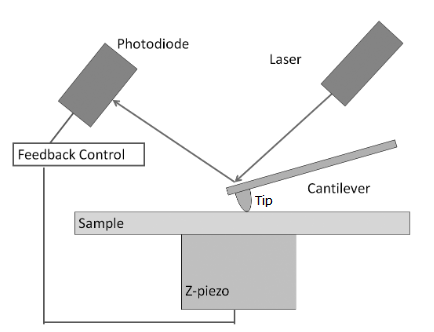
\includegraphics[width=110mm]{chapter2/RAFMSch.png}
\end{center}
\caption{A basic schematic of an set up AFM. Image adapted from \cite{RAFMSchRef}.}
\label{fig:AFMSch}                 % Reference label to the figure.
\end{figure}


%use "origin" rather than "0,0"
The general schematic of an AFM is shown above (figure \ref{fig:AFMSch}). The only directly interacting point upon the sample is the tip (which is mounted on a cantilever), keeping the interaction between the sample and mechanism to a minimum. A laser is emitted and aligned to the head of the cantilever above the tip. This laser is then reflected off the back side of the cantilever into a photodiode which converts input light into an output electrical signal. Initially the laser is set up to reflect into the origin position (the center) of the photo diode. This ensures that it has the maximum amount of room to translate across the surface as the cantilever deflects. As the tip is brought into contact with the surface the cantilever bends and relaxes as it processes over the sample. These translations alter the reflected angle off the cantilever, depending on the underlying sample surface topography. This reflected light then changes the positioning of the detected light on the photodiode, translating its x, y component relative to the alterations of the cantilever. The cantilever itself is moved across the surface by a piezoelectric motor with a high degree of precision. In some implementations, the piezo is singularly used to control the height position (z axis) of either the stage, or the tip. However, particularly in imaging mode AFMs, the piezo can additionally accommodate lateral and horizontal (x and y axes) movement. Generally, an emphasis on accuracy is placed on z-axis sensitivity (with most AFMs citing the operational error on the z-axis to be within the order of magnitude of an \AA{}ngstrom, whereas the x/y-axis component error is within a nanometer). From this basis, the accuracy of the piezo controller may be one of the more important capabilities of any AFM, as all data and features fundamentally rely on fine position control and piezovoltage output readings. The piezo controller fundamentally controls the rate in which the AFM can operate as well. 
%citation about x, y a nd z

The feedback mechanism from these position controls relies on a laser reflected off the back of the cantilever. To aid this effect, the back of the cantilever is coated in a reflected material, such as gold or antimony. As the laser is reflected off and detected using the photodiode the changes from origin are measured and fed into the feedback control system. It is this feedback mechanism that directs the piezo's movements in the next cycle, as it controls the force applied on the surface. Generally during imaging the force applied is set to a specific magnitude, with the controller aiming to keep that constant across the whole operation. Movement across a whole dataset can vary depending on the type of operation being performed - such as imaging recording across a 2d area, and force profiling recording across a single x, y point in sample space.

Additionally, the cantilevers themselves have a wide range of options in terms of their properties. The spring constant, the length of the cantilever, geometry, tip shape, surface chemistry and more are some of the options that a operator has to consider. In some cases, the chip that the cantilever is attached to has multiple different cantilevers off the end of it, allowing a range of cantilever parameters, either to determine the best one for the case, or for probing a range of conditions. The spring constant and the length of the cantilever is used to control the cantilever's sensitivity to smaller forces (as force will bend a softer cantilever more than a hard one), or for probing surfaces. The geometry of the cantilever can be used to control for any rotation or lateral bending the cantilever may be subjected to, or for use in cases where a specific shape is needed. For example, a V shaped cantilever prevents any flexing or bending laterally.

Tip shape is also another consideration for operators as it can influence the output data. If a tip is unable to physically reach a portion of the sample due to steric interference then that portion of the sample is measured as an imprint of the tip's surface. Figure \ref{fig:tipshape} shows an example of two tip types interacting with a pit on a sample. The circular one is unable to enter the pit fully, giving a circular artifact equal to its imprinted geometry instead, whereas the triangular one probes the depths fully, giving the correct output impression. These sorts of gaps can also influence the forces felt by a tip as it interacts with it, as a ``gap'' of sample will not provide the expected sum of interactions.
%"probes the depths?"

\begin{figure}[h!]     %Insert a figure as soon as possible
        \begin{center}
          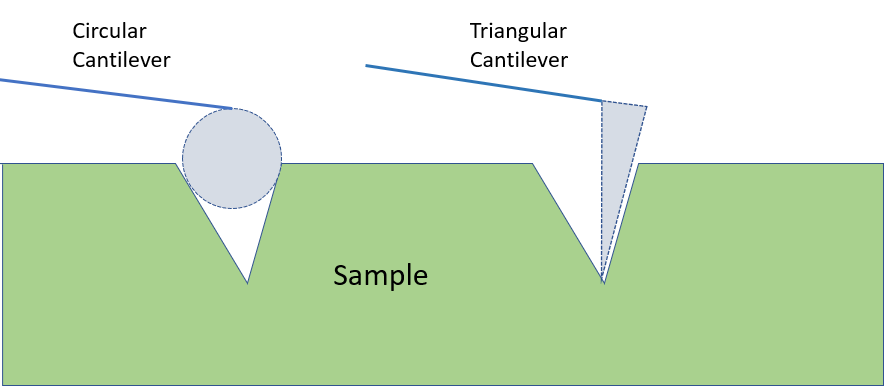
\includegraphics[width=110mm]{chapter2/Tip Shapes.PNG}
\end{center}
\caption{Above is shown the difference between tip shapes and types - where the tip with a circular geometry on the end is unable to enter fully into the crevasse on the sample, the thinner triangular one is. As a result, the output image/data will differ between the two tips, while the underlying structure remains the same, potentially leading the user to incorrectly interpret data.}
\label{fig:tipshape}                 % Reference label to the figure.
\end{figure}

As this tip is brought into contact with the surface it is subjected to various forces. As an example the total force applied to the cantilever is a combination of van-der-Waals attractions and electrostatic repulsion as described in chapter 1. The resultant force scales with the separation distance of the tip from the surface, \textit{h}. When the tip is in direct contact with the surface, the  elasticity of a surface can be directly probed. When the tip is physically in contact with the sample, piezo movement into the surface is directly translated into bending as the cantilever is forced away. This process can also be used to determine the elasticity of surfaces by intentionally pressing the tip into a surface.

For the majority of AFMs in use today, the raw unprocessed data given by a machine boils down to the piezo extension and position of the reflected laser on the photodiode, as well as the piezo's z positional height, which is tied to its total operational range. This data is fed into the feedback control loop in order to adjust the tip's position to stay within operational parameters. This process is tied to the software's main cycle loop time, which occurs faster than the operator can respond to it - on the order of miliseconds, or even less. The operator instead of having a direct involvement in the cantilevers positioning and control instead sets boundaries for a range of variables depending on the operation type, but in general the speed, the force applied to the surface and the operational window (the start distance to intended end distance).

\begin{figure}[h!]     %Insert a figure as soon as possible
        \begin{center}
          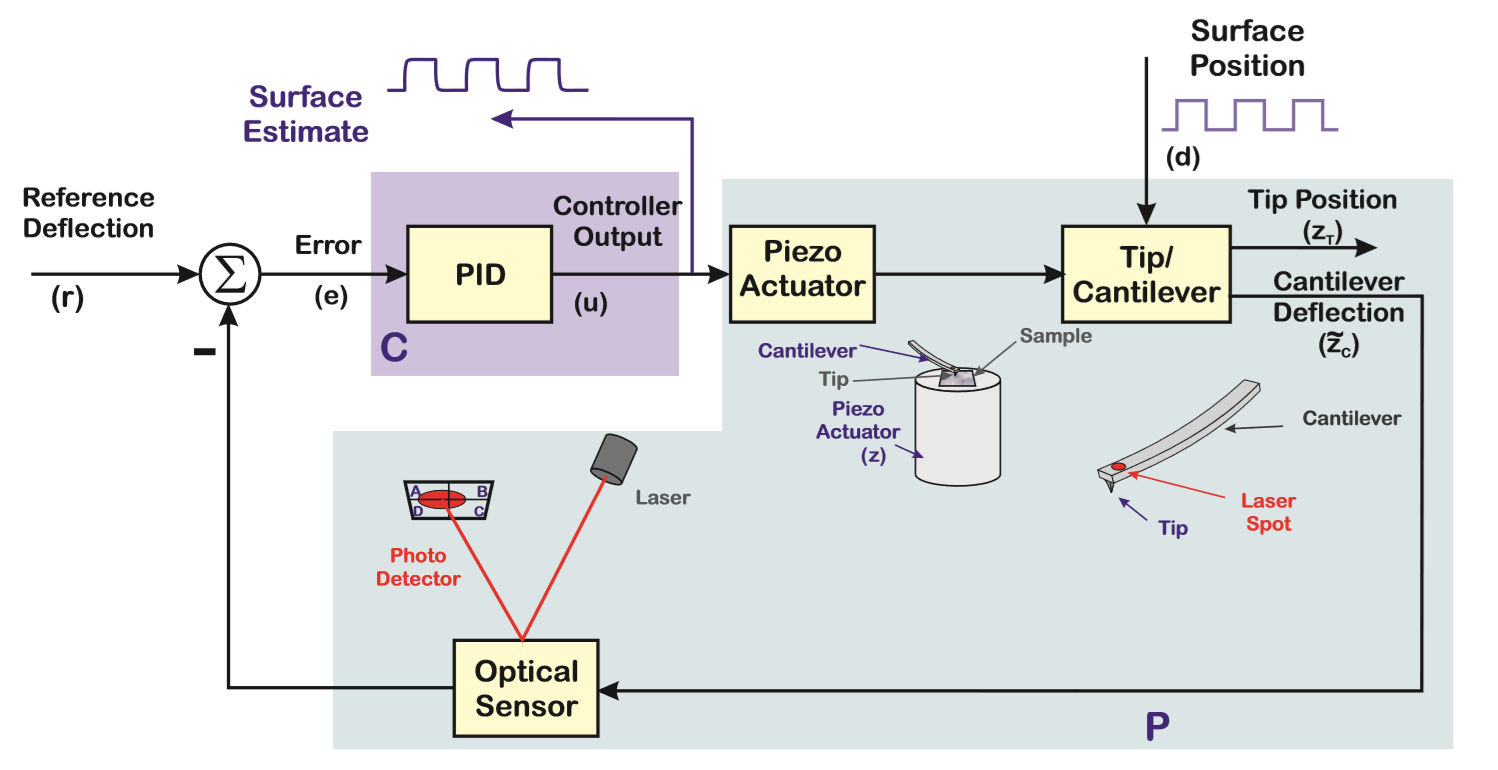
\includegraphics[width=110mm]{chapter2/Feedback.png}
\end{center}
\caption{A diagram demonstrating the basic feedback loop control for an AFM. In this case an example for an AFM operating in imaging scanning mode is shown, which is elaborated in the next section. Image adapted from \cite{AFMTut}}
\label{fig:Feedback}                 % Reference label to the figure.
\end{figure}

From these parameters, the cantilever is controlled in a feedback loop. First a reference signal is generated and cross referenced against the cantilever deflection. From this the gain is tweaked to attempt to apply a constant force to the tip across measurements (known as the setpoint).

%\begin{figure}[h!!!]     %Not needed anymore - too indepth into mechanics.
%        \begin{center}
%          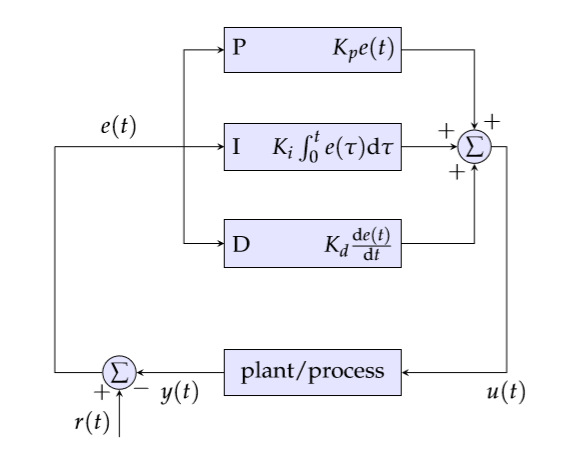
\includegraphics[width=110mm]{chapter2/PID.PNG}
%\end{center}
%\caption{A basic schematic of an PID-controller circuit where \textit{r(t)} is the setpoint, \textit{y(t)} is the reference signal and \textit{u(t)} is the difference. \textit{P} calculates the weight of the error signal input, \textit{I} weights the sum of previous errors and \textit{D} calculates the change in error over time to predict future errors. Image adapted from \cite{GoodAFM}.}
%\label{fig:PID}                 % Reference label to the figure.
%\end{figure}

From this loop, the tip position and the cantilever deflection is recorded. This loop helps to ensure that a constant force is applied to the tip, to reduce tip and sample damage as well as the reduction of errors in the system, as AFMs usually operate at a rate faster than human control. \cite{GoodAFM}\cite{AFMTut}

%The cantilever itself 

Using this loop the tip can then be exposed to various ranges, with corresponding forces acting upon it. These ranges are used to define various modes of operation such as: contact mode; where the tip comes into full contact with the surface, tapping mode; where the tip only lightly grazes the surface and non contact mode; where the tip is only affected by the long range forces. As you move the tip further away from the surface the force applied on the surface is reduced, which is particularly useful for softer samples. For force curves however, the force measured is generally across the spectrum. \cite{GoodAFM}\cite{AFMTut}

\begin{figure}[h!!!]     %Insert a figure as soon as possible
        \begin{center}
          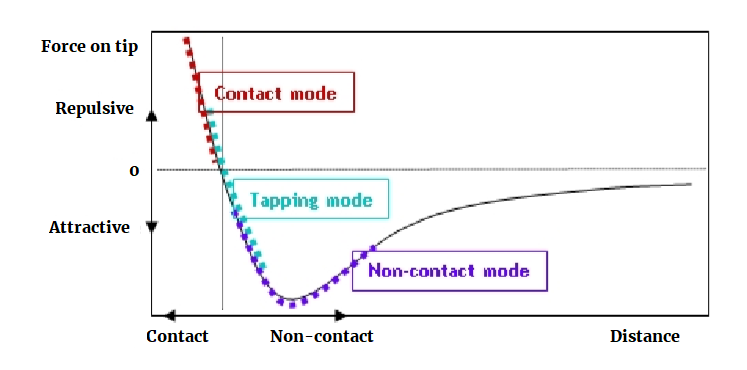
\includegraphics[width=110mm]{chapter2/Regions.png}
\end{center}
\caption{A Van-der-Waals potential with corresponding regions imposed over the curve to demonstrate the ranges each of the modes have in relation to the forces applied to the cantilever. Image adapted from \cite{GoodAFM}.}
\label{fig:Regions}                 % Reference label to the figure.
\end{figure}

For the non-contact modes the probe is set to oscillate at the resonance frequency of the cantilever. When the tip comes close enough to the sample to be affected by the surface forces it causes a dampening of the oscillation, resulting in a phase shift. Using this method, the speed and accuracy of mapping is improved. Tapping mode is similar, except that the nadir of the oscillation is brought into contact with the sample.

From these methods and mechanisms AFM has branched out into performing a range of functions, the two most common being imaging and force profiling which rely on this tip-surface interaction to generate the surface and interaction profiles of samples respectively.

\section{Tip Calibration}
\label{chap:cali}

Tuning a cantilever for use under imaging mode is generally one of the simplest methods of calibrating an AFM. By sweeping a cantilever over a range of drive frequencies a maximum peak of cantilever amplitude can be found. From this the resonance frequency is assumed. However issues can arise when calibrating a tip for use under liquid as the viscous drag of the liquid dampens the oscillations of the cantilever. As a result non contact methods are generally not applicable for imaging samples under a solution and rely on contact methods.

In general however, for cantilevers used in air the thermal noise spectra can be mapped to a simple harmonic oscillator, with a noise floor added to compensate for the baseline noise found in the system. This relies on the cantilever being longer than it is wide, and the the quality factor being greater than the sum of the oscillation. The power spectral density $PSD(\omega)$ as a function of angular frequency is a function that describes how the power of a signal or time series is distributed with respect to frequency.

The $PSD(\omega)$ is used to analyze the cantilever's thermal noise spectrum. The cantilever, when not being externally driven, will still oscillate due to thermal energy (Brownian motion). These thermal oscillations create a noise spectrum that can be analyzed to extract useful information about the cantilever, such as its resonant frequency and quality factor.

the $PSD(\omega)$ is given by:

\begin{equation}
PSD(\omega) = A_{white} + \frac{A_0 \omega^4}{(\omega^2 - \omega^2_r)^2 + \frac{\omega^2 \omega^2_r}{Q^2}}
\end{equation}

where $\omega$ is the Angular frequency, $\omega_r$ is the resonant angular frequency of the cantilever, $A$ is the Peak amplitude of oscillation, $A_0$ is a scaling factor for the peak amplitude, $A_{white}$ is the noise floor, a constant representing the baseline PSD, and $Q$ is the ratio of energy stored to energy dissipated in one cycle. The quality factor is a dimensionless term which correlates to how underdamped said oscillation is - i.e. it is the loss of energy across one oscillation period. 

Generally for imaging mode AFM the thermal tune method of calibration for cantilevers is adequate. One of the major benefits to this method is how it is non damaging to the tip and relies on the thermal energy driving the oscillation of the tip itself in air. From this the spring constant of the cantilever can be detected by using the equipartition theorem which relates the thermal energy of a cantilever to it's spring constant. The output value is then generally sanity checked by cross referencing with the manufacturer's ranges, or in the case of a cantilever created by the operator themselves, a more in depth calibration may be used. Calibration can also be used as a rudimentary method to detect damage to the tip during processing - as degradation of the tip will alter the oscillation of the cantilever leading to results outside of expectations. 

The spring constant of the cantilever is calculated using:

\begin{equation}
\frac{1}{2}k_{B}T = \frac{1}{2}kx^{2}
\end{equation}

Which can be simplified to:

\begin{equation}
k = \frac{k_{B}T}{\langle x^{2} \rangle}
\end{equation}

where k\textsubscript{B} is Boltzmann's constant (1.38064852 × 10\textsuperscript{-23} m\textsuperscript{2} kg s\textsuperscript{-2} K\textsuperscript{-1}) and T is temperature in Kelvin. x\textsuperscript{2} is distance in respect to the power spectral density (PSD), which is fit to the simple harmonic oscillator mentioned above. \cite{ThermalCalc, JankThesis}

\begin{figure}[h!!!]     %Insert a figure as soon as possible
        \begin{center}
          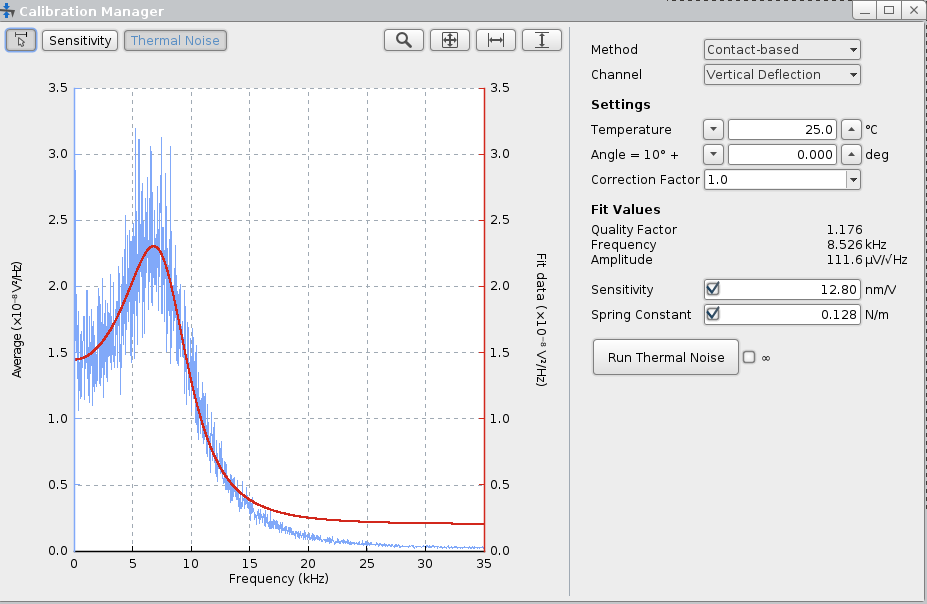
\includegraphics[width=110mm]{chapter2/caliEg.png}
\end{center}
\caption{An example of a thermal tuning calibration software interface.The blue line is the raw signal from the AFM and the red line is the fit over that data. The operation itself is automatic, requiring the user to only press the run thermal noise button for the spring constant to be given.}
\label{fig:caliEg}                 % Reference label to the figure.
\end{figure}

%cite yt vid Tbr8zjLywHI

%Copy paste From wiki do not uncomment: {The quality factor or Q factor is a dimensionless parameter that describes how underdamped an oscillator or resonator is. It is approximately defined as the ratio of the initial energy stored in the resonator to the energy lost in one radian of the cycle of oscillation.}
%Why do people hate defining their terms

After the laser has been aligned the system can detect changes in the cantilever, in particular bending. However, for this bending to be converted into force applied to the cantilever and/or surface, the system itself must be able to translate bending into force. Unlike imaging mode where the peak resonance is the main factor in determining a good calibration, the force instead relies more on a spring constant coupled with the inverse optical lever sensitivity (InvOLS). This is due to the force being calculated, rather than imaging producing a height map based off the cantilever deflection. In the case of force; 

\begin{equation}
F = kz
\end{equation}

where k is the spring constant of the cantilever and z is the cantilever deflection. The cantilever deflection is in turn calculated using:

\begin{equation}
z = InvOLS\Delta V
\end{equation}

Where $InvOLS$ is the Inverse optical lever sensitivity (m/V), and $\Delta V$ is the change in the voltage measured by the photodiode. $\Delta V$ is given as a raw value from the machine.

InvOLS is dependant on a range of different factors such as spot size, position, cantilever length and electronic gains in the system, however this calculation can be bypassed by taking the slope of the curve on a hard surface, then finding the difference needed to convert said slope to be equal to one (Figure \ref{fig:InvOLS}). 

\begin{figure}[h!]     %Insert a figure as soon as possible
        \begin{center}
          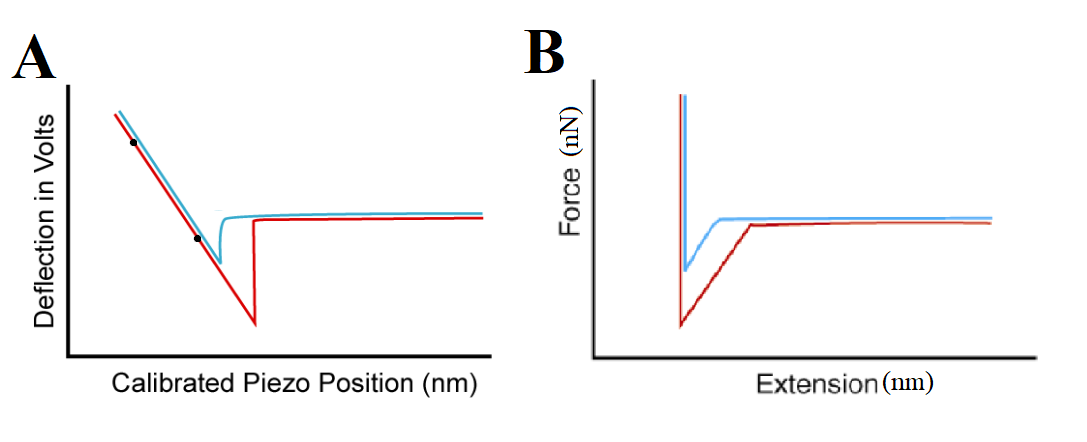
\includegraphics[width=100mm]{chapter2/InvOLS.png}
\end{center}
\caption{A diagram demonstrating the translation of InvOLS to force, A demonstrates the raw data plotted, B demonstrates the data adjusted with InvOLS into a force. Adapted from \cite{AFMTalk}}
\label{fig:InvOLS}                 % Reference label to the figure.
\end{figure}

Both of these methods assume that cantilevers are motionless, or do not contribute any motion to the input motions dictated by the piezo controllers. In reality this is not the case, as cantilevers are always moving. Even a baseline measurement of lever deflection will deviate by 2 nm in vacuums, air and water by thermal noise.\cite{AFMTalk} \cite{AFMCalibration, AFMCalibration2}

%https://nanohub.org/resources/11221/download/2011.02.17-AFM_Workshop-L03-Moshar.pdf

% Add review here. - what review???

%Calibration of the cantilever is required to convert the raw signal produced from the AFM into force data. While an AFM under imaging mode may only need a thermal power spectral density graph plotted

%There are several parameters that can be controlled during force operation that affect the 



%\textcolor{red}{Sader method?}

\section{Common artifacts in AFM}
\label{chap:commonArtifacts}

One of the greatest strengths of AFM can quickly turn into a double edged sword in the wrong hands. Due to how the AFM physically interacts with the surface this means there is a lot more potential for unexpected interaction and unique artifacts when compared with traditional microscopy. Over the history of use of AFM certain recurring artifacts have been identified and recognised. These sources of artifacts in AFM generally come from either the tip, the scanner, vibrations, the feedback circuit, and the image processing software. 

\subsection{The tip}

The geometry of the tip is an important factor in AFM sample preparation and experimental design. this was briefly touched on earlier in figure \ref{fig:tipshape}. However there are further aspects to the geometry that can influence the results. These examples include when the tip itself is either damaged, contaminated or when the tip is dulled from excessive use. A damaged tip will cause an artificial shape up on the surface of the image as seen in figure \ref{fig:BrokenTip}. 

\begin{figure}[h!]     %Insert a figure as soon as possible
        \begin{center}
          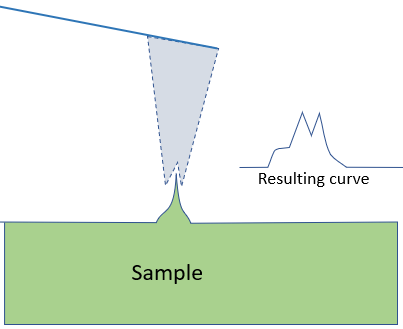
\includegraphics[width=100mm]{chapter2/BrokenTip.PNG}
\end{center}
\caption{As the damaged tip interacts with a sample surface an artificial lump is measured by the cantilever in scanning mode. This is due to the double prong defect in the probe head limiting the range of movement, incorrectly reporting a secondary feature.}
\label{fig:BrokenTip}                 % Reference label to the figure.
\end{figure}

Contaminated tips equally will affect results, but in an irregular way - as contaminants can be gained or lost during an operation. Whilst on a tip they alter the interacting geometry and chemistry of a probe. Additionally, these contaminants can change the surface profile of the sample, leading to inaccurate measurements. For example, if a sample was covered by a contaminant during force profiling, the resulting force curves would be altered by the contaminants interaction with the probe. Contaminants are generally very difficult to remove and usually require some kind of cleaning procedure to remove, hence the use of clean rooms for some sensitive AFM operations.
%this is fluffy - might be better in force curve section

A dull tip from overuse will decrease the sharpness and potentially the length of the tip - essentially widening it's interaction profile. This causes the interacting surface area to widen as well as widening any topology measured by the system. As such it's standard practice to regularly use fresh tips.
%Does this need an image?

Generally these sorts of artifacts provide a repetitive and unusual profile upon the surface, and can be checked by using multiple tips to profile the same sample. If the results are consistent across tips then it's unlikely to contain artifacts created by the tip itself.

\subsection{Scanner error}

The source of scanner error fundamentally derives from the piezoelectic scanner's physical properties. A piezo electric scanner will increase in sensitivity from constant use, or will slowly depolarise and increase in sensitivity when left idle. As a result, piezo electric scanners require regular maintenance to compensate for these effects. In addition to this phenomenon the extension of a scanner in any direction is not linear with its driving signal, which affects all z and x, y movements. When a piezo electric scanner is not properly calibrated this is usually reflected in dimensional distortion in the data. These sorts of artifacts have a constant presence and adjustment to any data generated and as such mandate the proper maintenance of any AFM. 

Correcting for these artifacts is either done by software or hardware and are usually not performed by the operator, instead handled by the manufacturer. Though nonlinearity effects are much less pronounced on the Z axis due to the reduced range of movement and these sort of effects only matter for very precise measurements when height profiling. 

Hysteresis is also a consideration when AFMs are cyclically scanned across a profile - these can cause a lateral shift along a trace and retrace curve causing an asymmetric step height. In the same vein rows can have drift, though this is due to a disconnect between in time steps between voltage driving movements. This usually presents itself as a bending drift across rows shown in figure \ref{fig:Creep}. Equally, this is why "zooming" into a scanned profile is difficult - these effects will displace the frame of reference by a certain offset when moving due to the change in cantilever scan velocity. 

\begin{figure}[h!]     %Insert a figure as soon as possible
        \begin{center}
          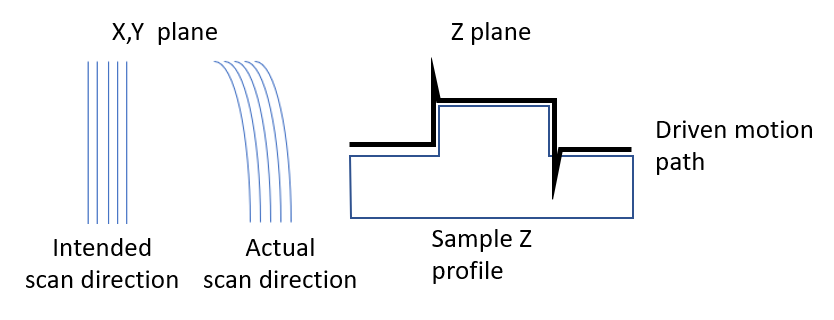
\includegraphics[width=100mm]{chapter2/Creep.PNG}
\end{center}
\caption{Creeping drift can occur across the motion of a scan. In the x, y direction this manifests as a bending motion, whereas in the z plane this can result in an overshoot of driven motion. In both cases the effects are exaggerated to convey the effects.}
\label{fig:Creep}                 % Reference label to the figure.
\end{figure}

%Too much detail - simplify? Maybe just spam images

In some cases of AFMs there is a parabolic arc attached to the x and y axis component of the piezo movement, which will cause bowling in the resultant image. Additionally, the sample itself cannot be atomically flat when inserted into the AFM. These two effects combine to cause an intrinsic tilt on the resultant image.

Finally thermal drift can cause changes in physical properties which will cause deviations from a thermally calibrated cantilever and the new properties. In the case of high resolution images small areas of thermal flux can cause issues, requiring the operator to wait until thermal equilibrium is reached.

The majority of these effects are dealt with either by hardware/software compensations outside of the standard use of AFM. During the data interpretation phase several mathematical transformations are performed on the data set to adjust for these effects.

\subsection{Vibrations}

Vibrations in the building, either due to foot traffic, wind, or even speech can cause physical displacements between the tip and sample. These vibrations can cause sudden shifts in the trace/retrace profile of a cantilever - leading to dramatic changes in the data. These are relatively easy to isolate as one time events however, and can be managed by operating the AFM in a quiet room with minimised background noise.

\subsection{Incorrect user parameters and feedback errors}

A large part of the AFM operation relies on the user to correctly set parameters during use. Generally these parameters are concluded during the operation to ensure that the output images are satisfactory. If incorrect parameters are set, then erroneous results can be easily produced. For example soft samples' profiles may be incorrectly compressed from a contact force too high, leading to a shorter than true height. As part of the feedback and correction mechanism relies on these input parameters the automatic corrections can further conflate errors in the resulting dataset.

For the majority of cases these artifacts are ironed out and compensated for over the course of sample familiarisation and as a result AFM tends to have a higher difficulty curve when compared to other microscopy techniques. Whereas other microscopy techniques will generally provide some sort of visual representation the sample imaging, improper use of AFM can result in phantasmagorical images without the appropriate care and consideration, leading to incorrect conclusions. \cite{AFMBook1}
%I really like the use of phantasmagorical here, but will it survive the review process?



%This whole section is spotted throughout with the orange book - cite it


\section{Imaging mode AFM}

Imaging mode focuses on using the AFM operation to measure the z-height of a sample across an x, y scan range. The positions are recorded in a three dimensional array, with the distance between each x, y entry value being constant. The major operation is much the same as described above, with the requirement of a piezo controlling x, y movement as well as z movement. The surface of the sample is imaged across using a raster pattern. This raster motion attempts to keep the respective z height at a specific force/deflection value as it progresses along the surface. In the case of non contact or tapping methods the oscillation dampening effect is kept constant across each position. The resultant array is often converted mathematically into a height map to display the surface profile of the imaged sample. 

Some AFM setups also provide other images during scanning; a phase image, an amplitude (or deflection) image and a friction image depending on the operational mode of the AFM. Generally two operational modes are available for the operator; contact and non-contact mode. Contact mode physically brings the tip in contact with the surface, then drags it across the surface. This is useful for measuring friction, reducing current effects on the tip in a liquid AFM situation and physically interacting with surface objects on the nanoscale. However this does have a shear force effect on the sample, and can damage particularly sensitive samples, such as biological material. Non-contact mode oscillates the cantilever above the surface, only allowing the tip to touch the surface gently at the nadir of the oscillation. By subtracting the input oscillation from the physical oscillation of the cantilever the phase can be determined. This indicates the softness of a surface, as harder surfaces dampen the movement to a greater degree, reducing the angle of the reflected laser.

\begin{figure}[h!]     %Insert a figure as soon as possible
        \begin{center}
          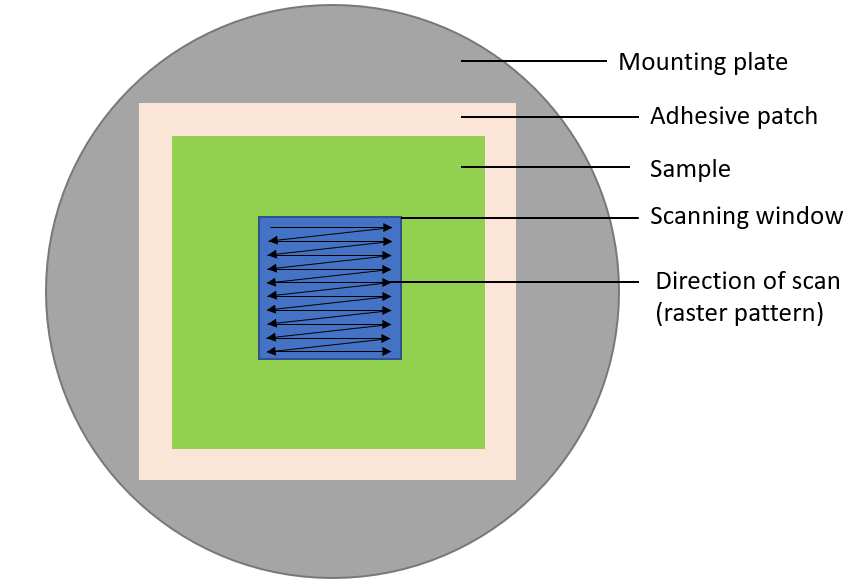
\includegraphics[width=100mm]{chapter2/SampleExample.PNG}
\end{center}
\caption{A diagram demonstrating the model setup for a sample. The geometry of each of the layers in the sample setup is an example in this case and can vary with application and requirements. The scanning window is non physical and is a projection of the area scanned by an AFM upon the surface of a sample.}
\label{fig:SampleExample}                 % Reference label to the figure.
\end{figure}

During use the operator defines a field of view (aka the scanning window) -  a range of coordinates that the AFM will take points of. This field of view is then broken up into number of points per line, which defines the aforementioned distance between each data point.

The raw export data is generally saved as a file, either to be adjusted in software or externally. This final data export however isn't reflective of the surface profile yet however - as the geometry and the local angle of the surface will alter the resultant output array. To compensate for the drift in the AFM and for the angle of the surface below the cantilever probe a few mathematical transformations are generally applied.

\subsection{Mathematical alignment and error correction of AFM images}

The use of AFM has proliferated across the sciences due to its wide range of applications and data output. However in some cases the image produced is assumed to perfectly reflect the surface of the sample, when in reality there are a number of mathematical, physical and operational effects that can vastly affect the output image. Mathematical transformations are applied to the raw data via image processing. Physical errors can occur from the situations the tip is exposed to and the condition of the tip. Finally operational errors can occur from improper use. As a result it is important to consider where these transformations and errors can arise to ensure that the image produced from the machine is a reflection of the true surface of the sample.

A part of the image processing process is done to compensate for the unavoidable artifacts discussed in \autoref{chap:commonArtifacts}. However this can be a source of error itself, as over reliance on multiple correction methods can introduce artificial profiles into the image. Other filters, such as a low pass filter can smooth out or remove sharper features in a data set. As such it is important for the operator to justify and consider any transformations upon the underlying data set.

%Example of "bad" paper with obvious tip defects/poor analysis? Can I even call out people like that?

\begin{figure}[h!]     %Insert a figure as soon as possible
        \begin{center}
          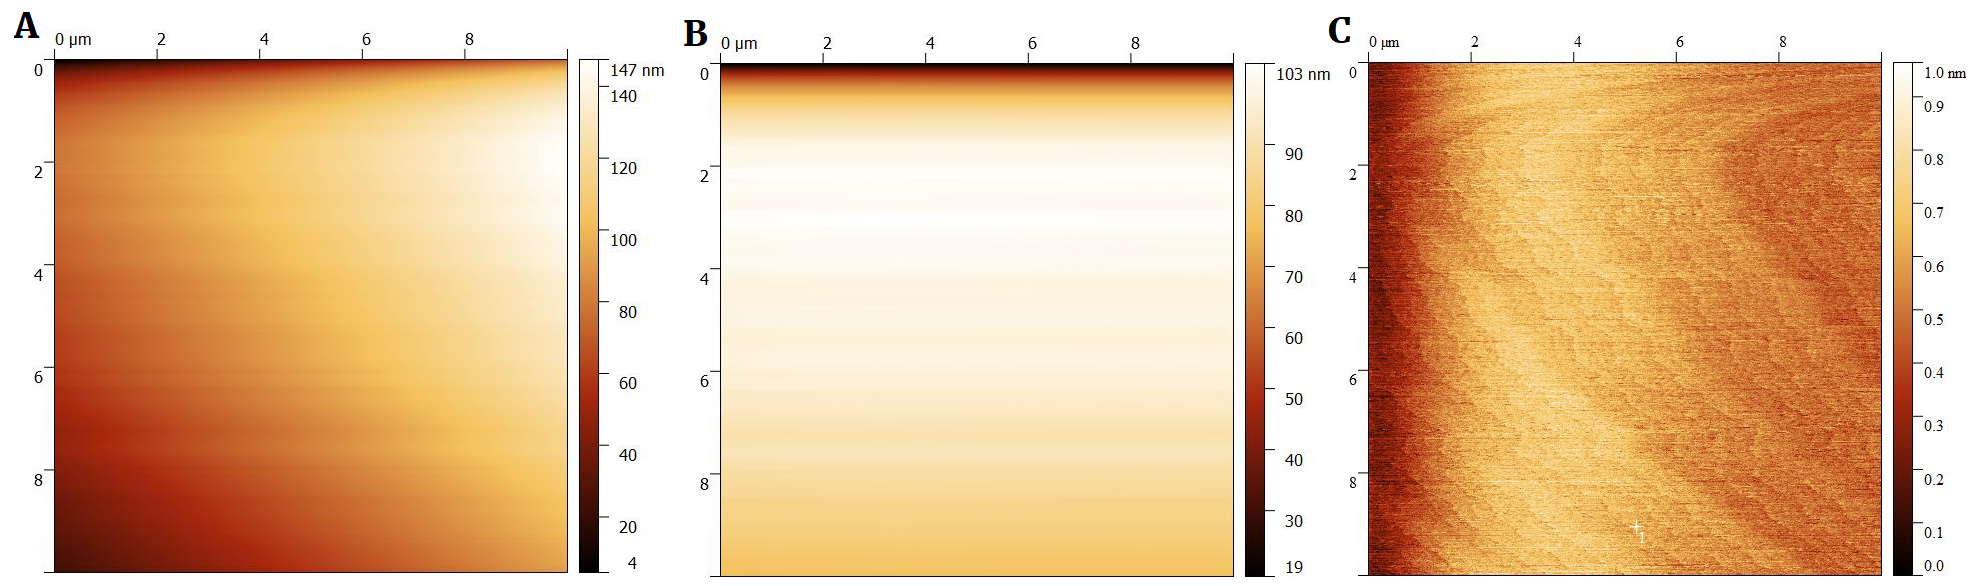
\includegraphics[width=140mm]{chapter2/MathOp.png}
\end{center}
\caption{A figure demonstrating a standard mathematical operation applied to raw data. A demonstrates the array shown direct without any processing, B has had a mean field plane subtraction applied and C has had a row alignment applied to it. The image itself is of a freshly cleaved mica surface which is reflected in the final image C.}
\label{fig:MathOp}                 % Reference label to the figure.
\end{figure}

Mathematical operations are performed on all images as the data generated does not account for the tilt of the surface, therefore a degree of mathematical transformation is required. Initially a heatmap of the the output will look similar to Figure \ref{fig:MathOp}. A mean field plane subtraction is used to determine the plane on which the data was generated, this is then removed across the dataset. This is to normalise the raw height data on a theoretical flat plane as an attempt to remove the tilt present on the sample stage. Next the rows of data are aligned by taking the representative height of each row and aligning each row to that height, this is done by several different methods, such as polynomial or median methods. As a result the features on the surface of a sample are kept intact, but it is possible that sharp differences observed on a row by row basis can be obfuscated due to image processing. The size of a pixel is dependant on the scan size (for example a 10$\mu$m by 10$\mu$m image with 512 data points per line means that each pixel is approximately worth 20 nm). Though, this does not represent the interacting surface area between the tip sample surface. In order to reduce errors like these and to resolve features that may be hidden by pixel weight larger scan sizes are often coupled with smaller scan sizes to give both the larger order topography with the smaller detail analysis. It is important for an user to not perform too much image processing without explanation and reasoning as each additional correction can be a further abstraction from the truth.

\begin{figure}[h!]     %Insert a figure as soon as possible
        \begin{center}
          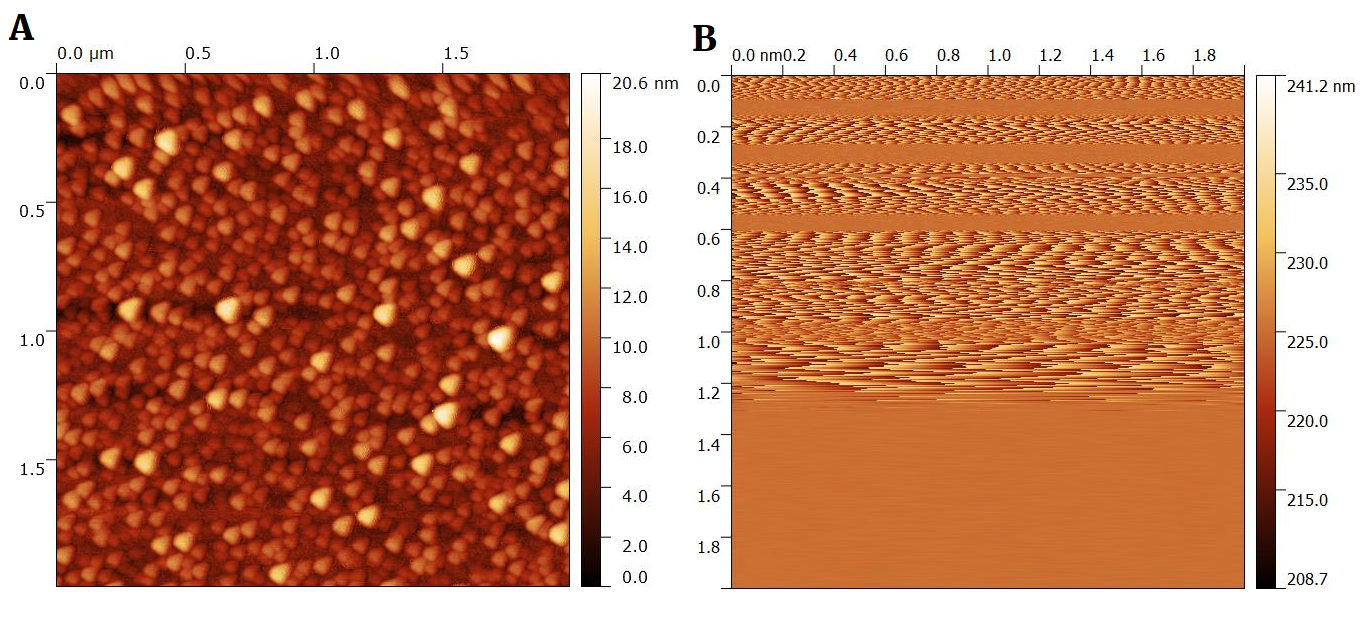
\includegraphics[width=140mm]{chapter2/Error.png}
\end{center}
\caption{A figure demonstrating different errors and operations on the output images produced from an AFM.  A.  demonstrates  a  physical  complications produced by contaminants on tip damage.  B. highlights an example of the zigzag patterns that can be produced from operation error, as well as the blank areas where the tip is not in contact with the surface.  }
\label{fig:Errorr}                 % Reference label to the figure.
\end{figure}

Another consideration with AFM is that since the image is scanned over time rather than instantly there is a degree of physical error introduced during operation. Thermal fluctuations, piezo-error, vibrations and air fluctuations. Generally the error of an AFM in imaging mode is given to be +/-1 nm on the x and y length scale and +/-1 \AA{}ngstrom on the z length scale. Issues are made worse within liquid conditions where current effects induced by probe movement, vibrations, sample setup and approaching the surface can frustrate results. The change in refractive index in the liquid means that the laser has to be realigned and re-calibrated in more difficult conditions. Additionally it is important to assess images produced for unusual mechanical errors, such as the double tip effect, where the tip becomes damaged during scanning and the defect in the tip's geometry is reflected onto a sample. There runs the risk of papers being published with potential double tip effects within their AFM analysis to an unknowing operator, the double tip effect is shown in Figure \ref{fig:Errorr}.A.

The operator is able to adjust several variables whilst operating an AFM. How much force is exerted on the surface as a result of the tip's proximity is altered; too light and the output image is unclear, but  increasing force causes increased tip degradation rate. The scan rate is how fast the AFM scans, faster speeds increase image production, reducing the effects of drift, piezo error and thermal fluctuations. However, a high scan rate can result in unclear images and an increase in tip degradation. Finally gain can be adjusted, the values of which vary on the sample, setup and device. Images produced with incorrect settings can result in wavy mechanical patterns or poor image quality. An example of a tip that hasn't engaged the surface properly, therefore resulting in a poor pattern is shown in Figure \ref{fig:Errorr}.B. \cite{AFMBook2, AFMBook1}

%HMM maybe move house of horrors before
\section{Surface Force profiling}

Force microscopy operation of an AFM differs from imaging mode in that the x, y movement of the piezo is removed, and instead a static sample is placed underneath, with several curves taken of a single site. This uses the mechanical nature of AFM to quantify forces applied upon the tip of the cantilever. These forces cause the cantilever to bend away in the event of repulsive forces, or towards the surface in the event of an attractive force. The interacting surface chemistry and profiles of both the tip and sample determine these force interactions. This contact area is also influenced by the solution that this area is immersed in, such as ions within the solution screening charges between the two profiles.

Having an accurate spring constant of the cantilever is paramount for these kinds of operations, as the measured parameter is the deflection of the cantilever reported by the photo diode. This can be then translated into force using the calibration methods discussed in section \ref{chap:cali}. This is one of the reasons why calibration is still performed for manufactured tips with given spring constants.

\subsection{Anatomy of a force curve}

A force curve is fundamentally the force ``felt" by a cantilever as it is moved along a z axis. From this seemingly simple motion, several events commonly occur across this simple motion. 

\begin{figure}[h!]     %Insert a figure as soon as possible
        \begin{center}
          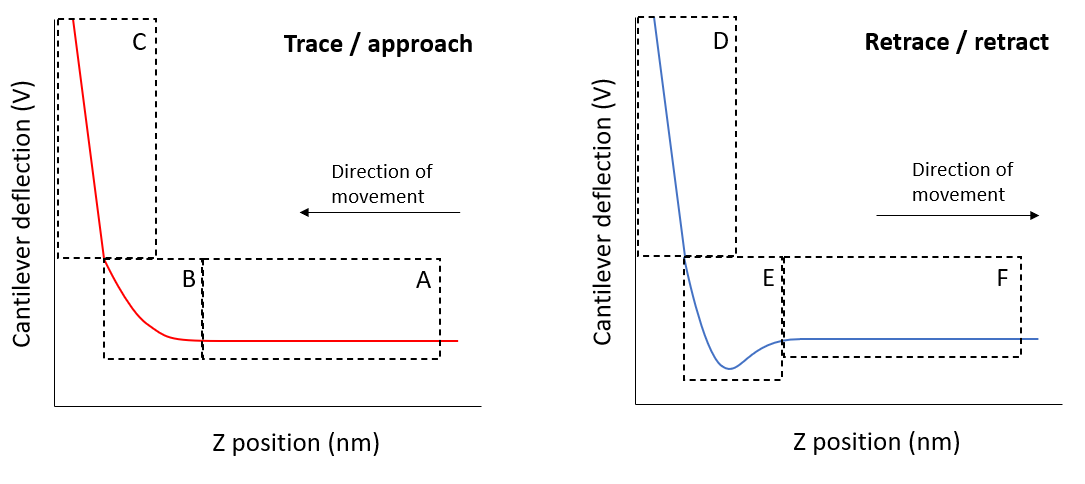
\includegraphics[width=140mm]{chapter2/forceCurveAnatomy.PNG}
\end{center}
\caption{A diagram showing a model force curve event. The leftmost image corresponds to the trace (aka approach) curve the first part of the force profiling event. The trace force curve proceeds from the bottom right up to the top left, passing through the A,B and C events in order. After this motion the piezo movement reverses, retracting the cantilever away from the surface, this begins the start of the retrace curve. In reverse fashion the cantilever progresses through the D,E and F sections in order.}
\label{fig:forceAnatomy}                 % Reference label to the figure.
\end{figure}

Given above in figure \ref{fig:forceAnatomy} is an unprocessed model force profile across one single scan. The first event labelled as A is the approach part of the curve - where the tip and sample are too far away for any forces to be detected by the cantilever. When the surface begins to apply force upon the cantilever it enters phase B; where the curve begins to bend away. This bending is indicative of a repulsive force between the two surfaces. When the cantilever is finally brought into contact with the surface the curve transitions into a linear profile, where any z movement is directly translated into deflection. The tilt intrinsic to this phase can be transformed away by converting deflection into force given in section \ref{chap:cali}.

In some cases it is possible for the operator to set a delay time to retain the tip upon the surface of a sample between the two curves. This is known as a delay period. Afterwards the retrace curve follow the same pattern a the trace, but in reverse, going through D,E,F. Region E indicates an attractive force between the sample and tip, bending the tip downwards. As these sample-tip bonds break the cantilever will snap up from the stress applied from bending. This can cause multiple snap up events if the interacting surface can unfold.

\newpage

\subsection{Error correction of force curves}

Since force profiling is restricted to a single axis in movement, the potential for error is reduced. The majority of artifacts and errors come from contaminants in the system, tip defects, or incorrect operational parameters. of particular note any error incurred by scanner artifacts such as drift is reduced when compared to imaging from the reduced dimensionality. Though one additional aspect does influence results that does not affect imaging mode - the relative topological differences between the interaction areas aka roughness. \cite{TipRoughness}

\begin{figure}[h!]     %Insert a figure as soon as possible
        \begin{center}
          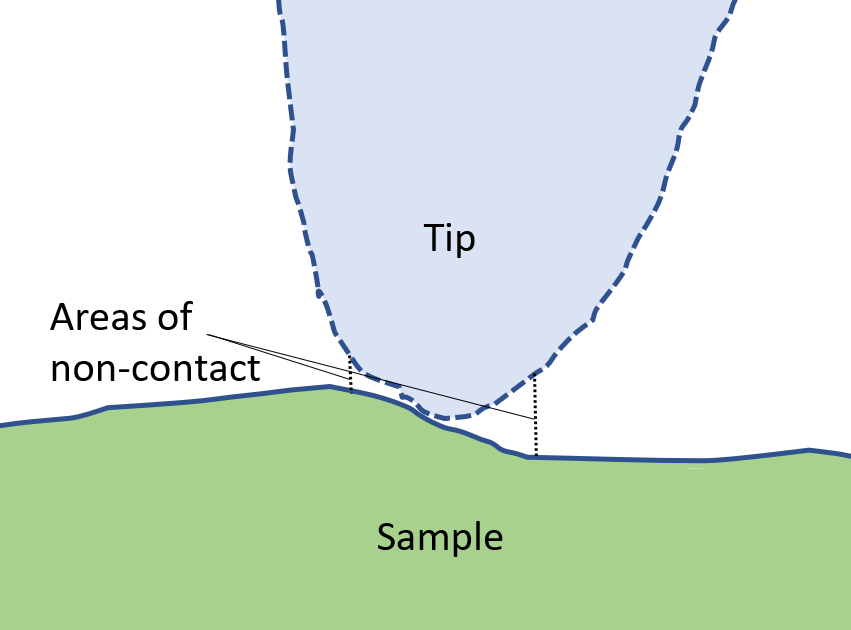
\includegraphics[width=100mm]{chapter2/tip contact.PNG}
\end{center}
\caption{A theoretical demonstration of a rough AFM tip interacting with an imperfect surface. Due to the differences in topology between the two surfaces the interacting areas generate a different sum force experienced by the tip than expected.}
\label{fig:tipCont}                 % Reference label to the figure.
\end{figure}

These differences can cause the sum force applied on the tip to be different than expected, leading to an adjusted force curve. This is due to the DLVO force profile resulting in different force effects along the different points within the contact area as shown in figure \ref{fig:tipCont}.
%Need better reference

In addition to this, because of the unstable geometry of the local area, as driving force increases, forcing the cantilever further into the sample, the tip itself can slip along the surface into a new more stable minima along the profile. This can cause sudden changes in the C/D regions mentioned in figure \ref{fig:forceAnatomy}. This effect is described in figure \ref{fig:tipSlip}. \cite{Ahmad2015}

\begin{figure}[h!]     %Insert a figure as soon as possible
        \begin{center}
          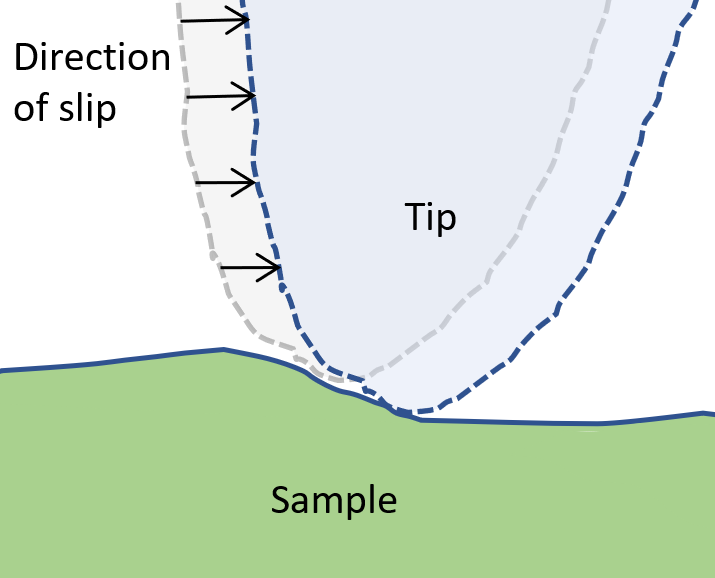
\includegraphics[width=100mm]{chapter2/tipslip.PNG}
\end{center}
\caption{A demonstration of the theoretical movement that a cantilever tip will undergo when slipping along a surface profile.}
\label{fig:tipSlip}                 % Reference label to the figure.
\end{figure}

To deal with these effects multiple force curves are generally taken across a range of sites to ensure that any localised profiles are averaged out.

One other consideration is the effects of hydrodynamic forces which will has a constant effect on the tip during motion (phases A/B and E/F in figure \ref{fig:forceAnatomy}). This only is present in samples immersed in a liquid, and generally doesn't impact the final curve too much. This effect can be profiled by running the machine in different driving speeds.

One other effect upon the resulting data profile is the driving speed of the cantilever during profiling. Depending on the measuring tick rate some nuance to the data can be smoothed out as a faster speed will have less time to measure each point in the curve. An operator will generally tune the machine and setup to find an acceptable middle ground between data points and time taken.\cite{AFMSurfaceProfile}
%Expand with a general overview


%\section{Application of Derjaguin approximation}
%moved to chapt 1

